\documentclass[bachelor]{INIAD}%卒論用 
\addtolength{\footskip}{8mm}
\bibliographystyle{jplain} 
%\usepackage[dviout]{graphicx}
\usepackage[dvipdfmx]{graphicx}
\usepackage{bm}
\usepackage{amsmath}

%\usepackage{geometry}
%\geometry{left=30mm,right=30mm,top=35mm,bottom=30mm}

%\documentclass[oneside]{suribt}% 本文が * ページ以下のときに (掲示に注意)
\title{象の卵生についての研究}
%\titlewidth{}% タイトル幅 (指定するときは単位つきで)
\author{東洋 太郎}
\eauthor{Taro Toyo}% Copyright 表示で使われる
\studentid{1F99999999}
\supervisor{赤羽台 花子}% 1つの引数をとる (役職まで含めて書く)
%\supervisor{指導教員名 役職 \and 指導教員名 役職}% 複数教員の場合,\and でつなげる
\handin{2021}{1}% 提出月. 2 つ (年, 月) 引数をとる
%\keywords{キーワード1, キーワード2} % 概要の下に表示される
\renewcommand{\baselinestretch}{1.25}
\setcounter{tocdepth}{2}

\begin{document}
\mojiparline{40}
\maketitle%%%%%%%%%%%%%%%%%%% タイトル %%%%

\frontmatter% ここから前文

%\etitle{Title in English}

%\begin{eabstract}%%%%%%%%%%%%% 概要 %%%%%%%%
% 300 words abstract in English should be written here. 
%\end{eabstract}

\begin{abstract}%%%%%%%%%%%%% 概要 %%%%%%%%
 ここには論文要旨を記述します。論文要旨の書き方については、指導教員の指導を受けること。
\end{abstract}

%%%%%%%%%%%%% 目次 %%%%%%%%
{\makeatletter
\let\ps@jpl@in\ps@empty
\makeatother
\pagestyle{empty}
\tableofcontents
\clearpage}

\mainmatter% ここから本文 %%% 本文 %%%%%%%%
\chapter{はじめに}
本研究の目的は,象の卵を発見して,象の卵生を証明することである。進化論的には,象は卵を産
む方が自然である。世界の動物園や,アフリカ,インドで空と陸の両面から多角的に探索を行う。
象の卵を発見した場合は,その形状の測定,材質の解析,工学的応用の可能性の検討を行う。

湯川による研究~\cite{yukawa1950quantum}では...

\section{なぜ象は卵を産むはずか}
今まで,哺乳類である象は卵を産まないとされてきた。しかし,哺乳類の定義は乳を与える動物
のことであり,必ずしも胎盤を持ち母親の体内で成長させる動物であるとは限らない。たとえばカ
モノハシは卵を産むし,カンガルーは体外の袋の中で新生児を育てる。哺乳類の動物が胎生か卵胎
生か卵生かは,進化上の分類よりもむしろ,生活の環境によって決まる。象のように大きく強い動
物の場合,重たい象の胎児を運ぶよりは,卵を産んでその重さから解放される方が楽である。また
卵が大きく硬い殻でできていれば,他の動物に取られたり食べられたりする恐れもない。さらに食
物を求めて象の群れが移動するときも,長い鼻で丸い卵を転がして行った方が,胎児を持ち運ぶよ
りエネルギー効率が高い。(恐竜も卵を産んだが,長い鼻を持たず,車輪を考案するだけの脳を
持たなかったため,巣を作った)こうした点から,象は卵を産む方が進化論的に自然である。

\chapter{関連研究}

\chapter{提案手法}

\section{象の卵の大きさ}
外形を計測し,それが絶対的な卵の形の枠であるアルキメデスの円筒座標表示形(式(\ref{Archimedes}))と一致するかどうか調べる。もし一致していなければ、卵でない可能性がある。
\subsection{サブセクションのテスト}
\subsubsection{サブサブセクションのテスト}
%%
%% 以下,番号つきディスプレイ数式モードの例
%%
\begin{equation}
r(z)=0.5\sqrt{1-(e^z-2)^2}
\label{Archimedes}
\end{equation}
%%
%% inline数式モードの例
%%
ここで,$r$は$z$軸からの距離,$z$は$xy$に直行する軸方向で,直交座標系は右手座標系であるとする。すなわち,$\hat{\bm{x}}$,$\hat{\bm{y}}$,$\hat{\bm{z}}$を,それぞれ$x$,$y$,$z$軸方向の単位ベクトルとしたとき,$\hat{\bm{z}} = \hat{\bm{x}} \times \hat{\bm{y}}$が成立している。
また,$r$の偏微分$\frac{\partial r}{\partial z}$は...
%%
%% 式番をまとめて表示する例
%%

ところで,カモメ(図\ref{kamome})が$x$羽,象が$y$匹としたときに,頭の数と,足の数の関係から,
\begin{eqnarray}
  \begin{cases}
    x + y = 2 & \\
    2x + 4y = 6 &
  \end{cases}
\end{eqnarray}

%%
%% 図の入れ方の例
%%
\begin{figure}[tb]
  \begin{center}
   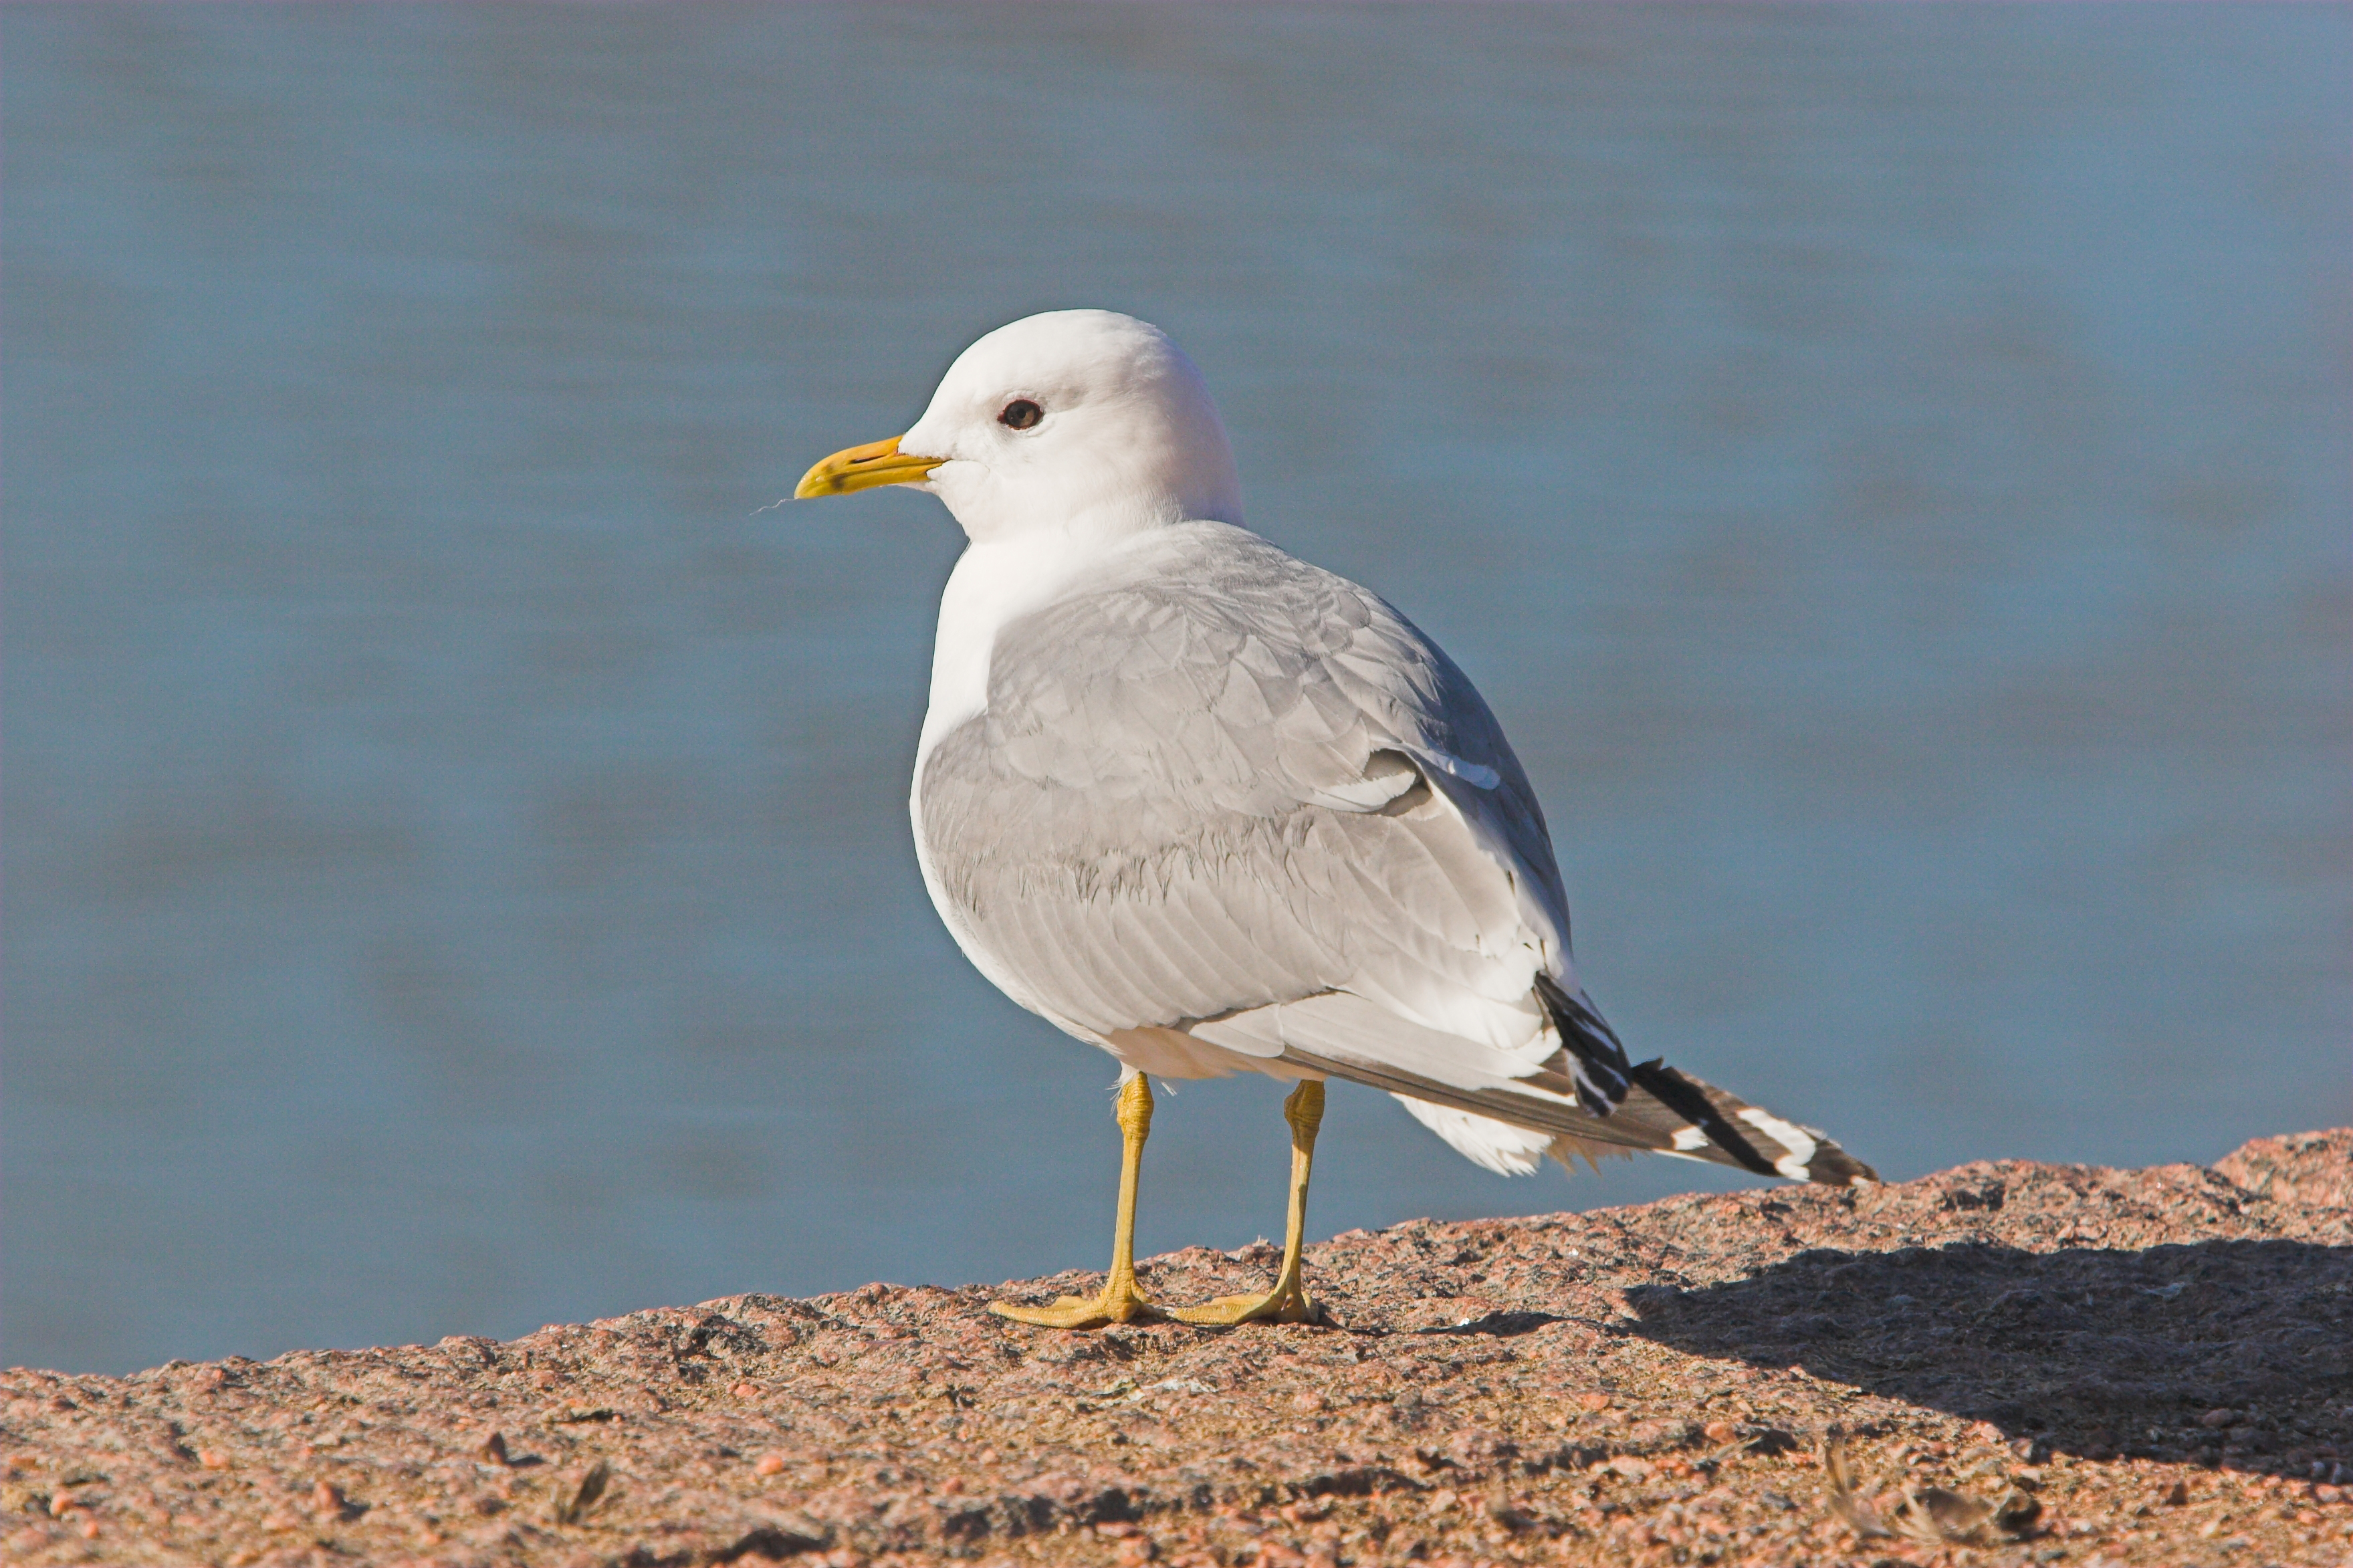
\includegraphics[width=0.4\linewidth]{image/kamome.jpg}
  \end{center}
  \caption{カモメ}
  \label{kamome}
\end{figure}


\backmatter% ここから後付
\chapter{謝辞}%%%%%%%%%%%%%%% 謝辞 %%%%%%%

% \begin{thebibliography}{}%%%% 参考文献 %%%
%  \bibitem{}
% \end{thebibliography}
%\bibliography{.bib ファイル名}% BibTeX を使う場合

\bibliography{thesis.bib}% BibTeX を使う場合

\appendix% ここから付録 %%%%% 付録 %%%%%%%
\chapter{}
\end{document}
